\documentclass[12]{article}

\usepackage{caption} 
\usepackage[hidelinks]{hyperref}
\usepackage{longtable}
\usepackage{times}
\usepackage{biblatex}
\addbibresource{kilder.bib}
\setlength{\parindent}{0pt}


\begin{document}{1.5}

\title{\textbf{\myfont{
            \HUGE Semester Project Group Report}}\vspace*{0.5em} \\
    \LARGE  University of Southern Denmark, Odense \vspace*{0.5em}\\
    \LARGE Faculty of Engineering}
\date{\today\vspace*{16em}}
\maketitle
\begin{center}
    \author{\large \textbf{Group 4}\\\vspace*{3mm}
        \vspace*{3mm}
        \large Benjamin Schmager Sørensen (besoe21@student.sdu.dk)\\
        \vspace*{3mm}
        \large Daniel Bermann Schmidt (dschm22@student.sdu.dk)\\
        \vspace*{3mm}
        \large Jonas Mathias Lissner (jolis22@student.sdu.dk)\\
        \vspace*{3mm}
        \large David Nielsen (davni22@student.sdu.dk)\\
        \vspace*{3mm}
        \large  Lukas Andersen (lande22@student.sdu.dk)\\
        \vspace*{3mm}\vspace*{3em}
        \large \textbf{Course code:} T500019101-1-E23\vspace*{1em}\\
        \large \textbf{Project period:} E23\vspace*{1em}\\
        \large \textbf{Supervisor:} Thomas Mørk\vspace*{1em}\\
    }
\end{center}

\maketitle

\thispagestyle{empty}
\clearpage
\pagenumbering{arabic}

\renewcommand{\contentsname}{Table of Contents}
\tableofcontents

\section{Introduction}

In this project we are working towardds creating an interface that can interact with a beer production machine using OPC UA. \newline

This interface needs to be user-friendly and be easy to use for anyone, as our primary targeted group is hobbyists, and other people who are interested in brewing beer. \newline
Aside from the viewable interface presented to the user, the program also needs features to make sure the production runs smoothly, and without major losses. \newline
This has to be done without needing a lot of input from the user, making it mostly automatic. \newline

\newpage
<<<<<<< Updated upstream
\section{Analysis}
=======
\section{Analysis}
\subsubsection{Personas}
In this project we decided to make some personas, to help us get an understanding of the systems capabilities and functionalities, they are fictional characters based on the stakeholder of the project. \newline

\begin{table}[htb]
    \begin{center}
        \begin{tabular}{|p{16cm}|}
        \hline
        \textbf{Kim, beer hobbyist} \\
        \hline
        \\ \textbf{Bio:} Kim is 42 years of age, he has a big patience for beers. It has been a big tradition in his family to brew their own beer, he recently decided that he wanted his own brewing machine to help him brew beer, he is not experienced in computers, so it must be user-friendly.  \\
        \\
        \textbf{Goal:} Kim is very excited to get his new brewing machine for his garage, he does have some concerns when it comes to the software part, he hopes that the brewing machine is easy to operate so that he can make beers when he wants too. \\
        \hline
        \end{tabular}
        \caption{Persona Kim}
        \label{tab:persona_kim}
    \end{center}
\end{table}

\begin{table}[htb]
    \begin{center}
        \begin{tabular}{|p{16cm}|}
        \hline
        \textbf{Lars, busy lawyer} \\
        \hline
        \\ \textbf{Bio:} Lars is 61, years of age. and works as a lawyer. he always works and dosent have a lot of time to spare, he has a passion for beers and would love to brew his own, his time is limited so the process of brewing should be simple and efficient.  \\
        \\
        \textbf{Goal:} Lars want to creat quality beer, without too much effort in the brewing process. He needs a machine that is user-friendly while also being effective. \\
        \hline
        \end{tabular}
        \caption{Persona Lars}
        \label{tab:persona_lars}
    \end{center}
\end{table}

\begin{table}[htb]
    \begin{center}
        \begin{tabular}{|p{16cm}|}
        \hline
        \textbf{Anna, Automation Enthusiast} \\
        \hline
        \\ \textbf{Bio:} Anna, 28, is an automation nerd, an always been impressed by machine that are automated, she is passtionate about beers, and have breewed some before manullay, but recently found interest in getting a automatic brewing machine for beers.  \\
        \\
        \textbf{Goal:} Anna aims to achieve tasty beers with only one click, which is selecting the beer she wants breewed with the new machine, she can get that, while alos having an automated machine. \\
        \hline
        \end{tabular}
        \caption{Persona Anna}
        \label{tab:persona_anna}
    \end{center}
\end{table}

\subsubsection{User Stories}

Now that we have requirements and personas, we can create some user stories. By creating user stories, we can make the program live up to the needs of the users.

\begin{table}[H]
    \begin{center}
        \sloppy
        \begin{longtable}{|p{1cm}|p{11cm}|c|c|}
            \hline
            ID & Stories & Estimation & Moscow \\ \hline
            US-1 & As a user I want the interface to be user-friendly, so that everyone can use it & 9 & M \\ \hline
            US-2 & As a user I want some already defined beers  so that I can select the beer I want without too much thought & 8 & M \\ \hline
            US-3 & As a user I want the brewing process to be automated so that I can click on a beer, it will start brewing & 7 & M \\ \hline
            US-4 & As a user I want the macine to handle difficulties automatically like maintenance so that I dont have to do anything & 8 & M \\ \hline
            US-5 & As a user I want to get displayed different data while the machine is brewing so that I can look at data & 5 & C \\ \hline
            US-6 & As a user I want the machine to be reliable so that I am guaranteed the beers is good quality & 6 & S \\ \hline
            US-7 & As a user I want the machine to be efficient so that I dont have to wait too long to get a beer & 5 & C \\ \hline
            US-8 & As a user I want the machine to be scalable so that I can add new beers to the machine & 4 & C \\ \hline
            US-9 & As a user i want the machine to have a quick repond time so that I dont have to wait for the machine to understand the input & 3 & W \\ \hline
            US-10 & As a user I want the machine to be able to handle different amount of beers so that I can choose the amount I want & 3 & W \\ \hline

            \caption{User stories for the beer machine}
            \label{tab:user_stories}
        \end{longtable}
    \end{center}
\end{table}
>>>>>>> Stashed changes
 

\section{Requirements}

Functional and non-functional\cite{example} requirements are listed in the table below. The requirements are based on the FURPS+ model, which is a model for classifying software quality attributes. The model is used to classify the requirements into different categories. The categories are functionality, usability, reliability, performance and supportability.
To give a better overview how the different non-functional requirements have been divided we have seperated each category of the FURPS+ model into different letters. Under the ID table R stands for reliability, U stands for usability, S stands for Scalability, P Stands for performance, and lastly the + for the spefic constraints in which contains Design constraints, Implementation constraints, Interface constraints and Physical constraints. \newline

The requirements are also classified into the MOSCOW model, which is a model for prioritizing requirements. The categories are must have, should have, could have and won't have. The requirements are listed in the table below. \newline

In the table below we have seperated each functional and non-functional requirements into the different categories in MOSCOW. M stands for must have, S stands for should have, C stands for could have and W stands for won't have.\newline

\subsection{Requirements using FURPS}
\begin{center}
    \sloppy
    \begin{longtable}{|p{1cm}|p{4cm}|p{8.5cm}|c|}
        \hline
        ID     & Name                       & Description                                                                                                                                                   & Moscow \\ \hline
        F-01   & Automated brewing process  & The beer machine needs to be able to automatically process the beer brewing process, through a user-friendly interface                                        & M \\ \hline
        F-02   & Recipe Management          & Users should be able to pick between different kinds of beer they want the machine to process.                                                                & S \\ \hline
        F-03   & Ingredients management     & The machine should automatically use the ingredients needed to brew a specific beer recipe.                                                                   & C \\ \hline
        F-04   & Alerts and Notifications   & Users should get alerts and notifications for the process if something fails or if the brewing of the beer was a success, or the machine needs maintenance.   & C \\ \hline
        F-05   & Data collection            & The system needs to collect data of the different processes to ensure we can improve the quality the brewing and minimize bad processing.                     & S \\ \hline
        F-06   & Cleaning and maintenance   & The machine should contain a cleaning and maintenance program to ensure that the quality of the beer is in top.                                               & M \\ \hline
        F-07   & Low failrete               & The machine must work in a speed that keeps the failrate below 1\% if possible                                                                                & M \\ \hline
        U-01   & User-friendly design       & To ensure that the process will be automated we need a user-friendly design with clear instructions and easy navigation to help the user brew beers.          & M \\ \hline
        R-01   & Reliability                & The beer machine should operate consistently and with minimal failures to ensure beer quality.                                                                & M \\ \hline
        R-02   & Data backup                & The data needs to be stores in a database to ensure no data will get lost from the brewing process.                                                           & S \\ \hline
        R-03   & Maintainability            & The design of the system should include well-documented code, modular design principles and meet industry-standard practices to ease future maintenance.      & S \\ \hline 
        R-04   & Separation of Concerns     & The architecture of the system should separate the concerns through multiple deployments to enhance maintainability, scalability and reliability.             & M \\ \hline
        P-01   & Performance                & It is important that the application has quick response times and minimal failures during the brewing process.                                                & M \\ \hline
        P-02   & Response time              & The response time of the application needs to be quick to ensure the user can navigate through the application without any delays.                            & M \\ \hline
        S-01   & Scalability                & The system should be able to scale if new recipes or features would be added to the machine.                                                                  & C \\ \hline
        S-02   & Future Development         & The program needs to be well structured, incase the application needs to be optimized or improved further                                                     & W \\ \hline
        

        \caption{Requirements using FURPS model}
        \label{tab:requirements}
    \end{longtable}
\end{center}

The Table \ref{tab:requirements} shows the requirements for the beer machine. The requirements are based on the FURPS+ model, which is a model for classifying software quality attributes. For a better understanding we have seperated each requierments into their own category and given them a Moscow priority.








% set the problem in context.
% summarise what you have done.
% describe your design solution.
% report on its performance.
% provide key recommendations.
\section{Design}
The project aims to develop a solution to automate and thereby ease the beer production process for the hobbyists, our design solution is strictly developed based on the previously mentioned personas and requirements.\newline
This process can under normal circumstances be a rather complex and very manual process, the user would have to manually control the temperature, add the correct ingredients and the right amount at the right time, while continuously monitoring the process to ensure that everything is going according to plan.\newline
The user might want to produce both produce multiple amounts, but also different kinds of beer. This would require the user to look-up each recipe every time to do the same recipe calculations based on the desired amount and beer type with every new batch, while monitoring and possibly adjusting the temperatures of the ingredients throughout the whole process for consistency.\newline
This process can quickly become overwhelming and tedious, especially for newcomers, and might lead to human errors as the production expands and in worst case, end up taking the joy out of the hobby.\newline
Our design goal is to make brewing easy and accessible to everyone, even for the least technical of people. We want to solve this issue by having a simple and clean user interface, without all the unnecessary information, where all the heavy calculations, continuous monitoring, and processing is done by software behind the scenes.\newline
The design aims to deter people from the seemingly advanced process of beer production by offering an intuitive and easy-to-use platform that removes the complexity and makes brewing accessible to every intrigued hobbyist.

\subsection{System Architecture}
The architecture of the system is based on the client-server model and include three deployments: The web-service, the database service, and the physical beer machine. \newline
The Web Service will consist of the front-end, back-end, and the OPC Client. There will be a direct line of communication between the user input in the user interface, through the data processing and handling in the backend, to the OPC Client that will handle the secure communication and instructions to the physical beer machine. \newline
The communication between the front-end, the back-end and the beer machine is implemented using a RESTful API. \newline
This deployment model ensures a clear separation of concerns, enabling efficient scaling in the future, while easing the maintenance of individual components.

\subsubsection{Frontend}
The user interface (UI) of the beer production system is developed using React, a powerful and easy-to-use JavaScript library with a lot of flexibility and efficiency in building interactive and dynamic user interfaces, which perfectly aligned with our goal of creating a user-friendly and responsive frontend for the beer production application.
In addition, Reacts offers a modular development environment in form of it's component-based design structure, this allows for the development of reusable UI elements, that can be combined to effortlessly form complex user interfaces. This helped the project to meet requirement U-01, to develop a user-friendly design, as each component can be developed and tested individually, before it's combined to form the final UI. \newline
The library also offers a virtual DOM (Document Object Model), which is a lightweight representation of the actual DOM, this allows for efficient rendering of the UI, as the virtual DOM only updates the necessary components, instead of re-rendering the whole UI every time a change is made. This helped the project to meet requirement U-02, to develop a responsive design, as the virtual DOM allows for efficient rendering of the UI, which in turn allows for a more responsive UI. \newline
Lastly it offered us a lot of flexibility in terms of state management, which is a crucial aspect of the project, as the UI needs to be able to handle a lot of different states, such as the different stages of the beer production process, and the different states of the beer machine. This helped the project to meet requirement U-03, to develop a dynamic design, as the UI can be updated to reflect the current state of the beer machine and it's progress. \newline
All these features, combined with the fact that it is a very popular and well-documented library, made it the perfect choice for the development of the user interface of the beer production system.
\subsubsubsection{User Interface}
To ensure we met requirement U-01, to develop a user-friendly design, we decided to develop a clean and simple user interface, without all the unnecessary information, to make it as easy as possible for the user to navigate and use the application. \newline
Therefore, an early draft of the user interface was developed to get a clear idea of the overall design and layout of the application. \newline
\begin{center}
  \centering
  \begin{figure}[H]
      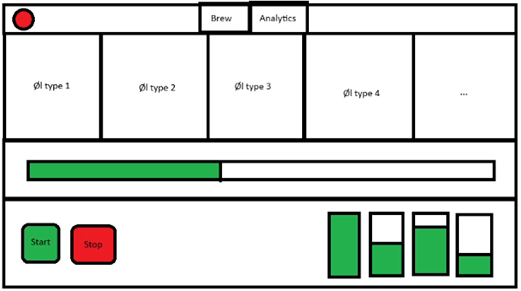
\includegraphics[width=1\textwidth]{img/frontend-draft.png}
      \caption{Early draft of the user interface}
      \label{fig:Frontend_draft}
  \end{figure}
\end{center}

\subsubsection{Backend}
The backend component of the beer production system will be implemented using Node.js, a versatile JavaScript runtime known for its efficiency in building scalable and high-performance server-side applications. Leveraging the strengths of Node.js, we aim to create a secure and reliable back-end that seamlessly communicates with the front end and the PLC-controlled beer production machine.

Node.js for Asynchronous Operations
Node.js excels in handling asynchronous operations, making it well-suited for scenarios where real-time communication and responsiveness are crucial. This feature aligns perfectly with the requirements of our beer production system, allowing for efficient communication between the user interface and the hardware components.

RESTful API Development
The back end will expose a RESTful API (Application Programming Interface) to facilitate communication between the front end and the PLC-controlled beer production machine. This API will define endpoints for actions such as initiating the brewing process, retrieving data, and handling alerts or notifications. Node.js, with its lightweight and fast I/O operations, is ideal for developing RESTful APIs.

Secure Communication
Security is paramount in the back-end design. Node.js offers robust libraries and modules for implementing secure communication protocols, such as HTTPS. This ensures that data exchanged between the front end and the beer production machine is encrypted, minimizing the risk of unauthorized access.

Data Storage with NoSQL Database
For efficient data storage and retrieval, a NoSQL database, such as MongoDB, will be employed. Node.js seamlessly integrates with NoSQL databases, offering a flexible and scalable solution for storing data related to beer recipes, production logs, and system configurations.

WebSocket for Real-Time Communication
To enable real-time communication and push notifications to the front end, WebSocket technology will be implemented using Node.js. This bidirectional communication channel ensures that users receive immediate updates on the brewing process, alerts, or any other relevant information.

Containerization for Scalability
In line with the project's emphasis on scalability, containerization technologies like Docker and Kubernetes will be utilized. Node.js applications can be efficiently containerized, providing a scalable and easily deployable solution. This approach ensures that the back-end infrastructure can adapt to increased load or additional features in the future.

Logging and Monitoring
Node.js provides robust logging mechanisms, allowing for the systematic recording of events and errors. Monitoring tools will be integrated to track the performance and health of the back-end system. This ensures that any issues can be promptly identified and addressed.

Testing and Continuous Integration
The Node.js back end will undergo thorough testing to validate its functionality, security, and scalability. Continuous Integration (CI) practices will be implemented to automate the testing process, ensuring that each code change is rigorously assessed for quality and reliability.

In summary, the use of Node.js for back-end development brings scalability, real-time communication, and security to the beer production system. By leveraging the strengths of Node.js, we aim to create a robust foundation that seamlessly integrates with the front end and effectively communicates with the PLC-controlled beer production machine.

\subsubsection{communication}
The communication between the front-end and the back-end is implemented using a RESTful API. 

\subsection{Simulation}
Incorporating the provided ARsim simulation tool early on into our development process was a crucial aspect of this project. 
The early integration allowed us to speed up the development time from the very beginning of the project, as most of our program's functionalities could be tested directly without the need for direct access to the physical machine.
As the tool allowed us to interact with ARsim in a manner similar to how our software would communicate with the actual hardware, it also enabled multiple people to test multiple different things without interfering with one another.
% ARsim serves as a valuable resource that enables simulation of the beer production process without the need for direct access to the physical machine. 
%This simulation tool will be instrumental in testing and refining our software application.

\subsubsection{ARsim Integration}
The ARsim simulation tool was integrated early into the development process, to mimic the behavior of the beer machine.
The early integration allowed us to speed up the development time from the very beginning of the project, as most of our program's functionalities could be tested directly without the need of the physical beer machine.
This integration also allowed us to interact with ARsim in a manner similar to how our software would communicate with the actual hardware, and enabled multiple people to test multiple different things without interfering with one another. 
% By leveraging ARsim, we can perform comprehensive testing of the software's functionalities, ensuring robustness and reliability.

\subsubsection{Testing Scenarios}


\subsection{Data Processing and Logging}

\subsection{Security Measures}

\subsection{Prioritization of Requirements}

\subsection*{Development Methodology}

\subsection*{Risk and Mitigation}

\subsection{Project Organization}

\subsection{Deliverables}
\section{Implementation}
To help us get a better understanding of the development process, we settled on using a software engineering practices called Agile methodology. By using Agile methodology in this project, it helped us to get a better overview of the overall product. The main reason to use agile methodology is that, you can always go back and change the requirements and functionalities of the software while developing.
In our case we had a stakeholder which is based on the persona, that was mentioned earlier. \newline
Reflecting on the implementation it gave us alot of knowledge and oppportunities to go back and change the the different functionalities to help us live up to the needs of the stakeholders, to make sure that the software was made for their specific use case, and help us stay in the scope of the project. \newline
To help us manage and optimize the develpoment process, we used Scrum, which is a framework that uses the same priciples as the agile methodology. The use of scrum helped us to stay organized, by splitting the project into smaller parts, to help keep track of what needed to be done.
We decided to split the project into five different sprints and each sprint was about two weeks time. By splitting the project into different sprints, we could get an overview of what needed to be done for that current sprint, while looking forward and seeing what needed to be done in the future.
While also seeing what did not get done in the current sprint. If a feature was not implemented in the current sprint, we could either delete it or move it to the upcomming sprint, this was very usefull to make sure that all functionalities and requirements where fulfilled.

\subsubsection{Technologies}
To help us develop the system, we decided to use some different software technologies that includes Docker, Node.js, React, OPC-UA. All the listed thing helped us develop the system the way we wanted it.
Docker is a containerization feture that allows us to run several applications in a single container. We decided to use docker to run the OPC-UA client, frontend and backend. By using the containerization technology we could boot the applications simultaneously, instead of running them seperate in their own file. This saved us alot of time and trouble.\newline\newline
The backend is developed in Node.js, which is a JavaScript runtime, with the Express package. The reason that we decided to use node.js was because the frontend is developed in React, which also is a javascript package. This helped us to get a secure and easy connection between the frontend and the backned without to much effort. The OPC-UA client is developed in javascript, with a package called node-opcua. This is an open source package that allows connection and communication with an OPC-UA server.\newline\newline
The reason we went with node-opcua instead of the provided MILO package in Java 8, was because, we already decided that we wanted to build in backend and frontend in javascript, and by using node-opcua we could use the same language for the OPC-UA client. This allowed us to establish a secure connections without failures, and it also allows us a better integrity of the system.
By using javascript for the overall structure of the system, we could ensure that the system is scalable and maintainable in the future. Aswell as not having multiple different programming languages in the system, which can lead to conflics and other problems. \newline

\subsection{Design Implementation}

\subsubsection{Architecture Implementation}
The implementation of the system is based on making a system that is rather easy to maintain and expand on in the future. We decided to use a container to run the backend, frontend and OPC-UA Client. This is done by using a dockerfile, that boots up the different containers.
by doing it this way, we can easiliy maintain and add features to the system. It also allows us to live up to the need of the user, where he only needs to click the beer he wants, and then the system will do all the things for him. \newline
To give a better understanding of the system, and the integrity, we made a deployment diagram, that shows how the system is deployed, and how the different components are conncted and talking to each other. \newline

\subsubsubsection{Deployment Diagram}
\begin{center}
    \centering
    \begin{figure}[H]
        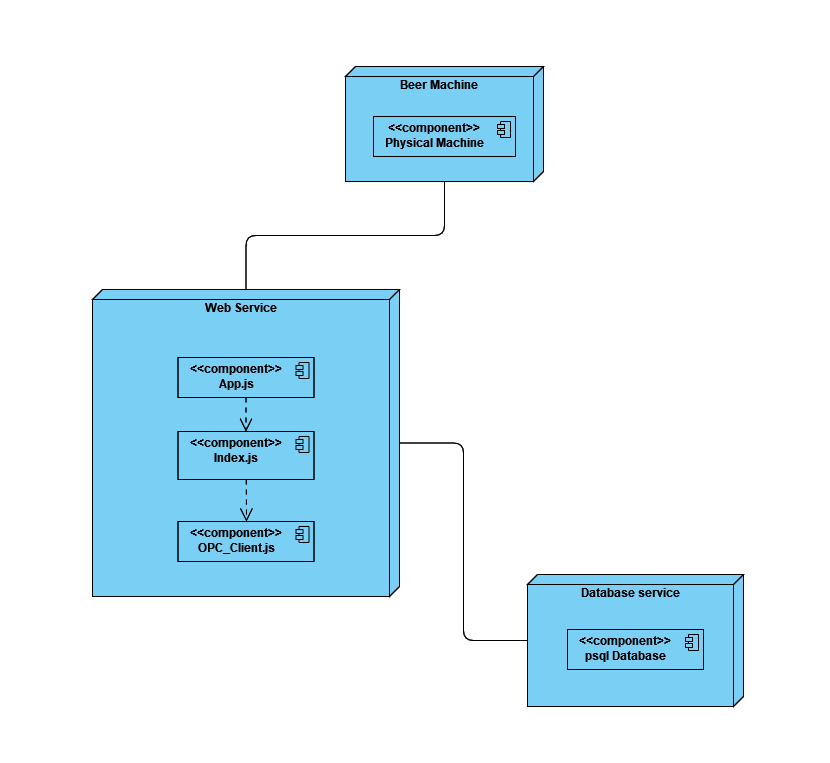
\includegraphics[width=1\textwidth]{img/Deployment_diagram.png}
        \caption{Deployment diagram over the system}
        \label{fig:Deployment_diagram}
    \end{figure}
\end{center}
Figure \ref{fig:Deployment_diagram} shows the deployment diagram of the system. The diagram shows how the different components are connected and to give a visual understanding of the system. The system is divided into three components, a dockerfile that boots up the backend, frontend and OPCUA-Client, we have the beer machine itself, and lastly the database which enables us to save data that is generated during the brewing process. This data collected can be accesed and help us understand and give improvements to the system. \newline

By deploying the system this way, we can ensure that the system is scalable and maintable in the future. it also enables us to add new features such as new beer recipes, or other things the client may want to help him brew beers. be encapsling the webservice into a container, we can make changes, updates and etc, which helps us reducing the risk of conflics with other parts of the system. \newline

\subsubsubsection{Sequence diagram}

Now that we have declared how the system is being deployed, its important to understand the realations/communication between the different application, in the following sequence diagram, we can see the interation between the application.

\begin{center}
    \centering
    \begin{figure}[H]
        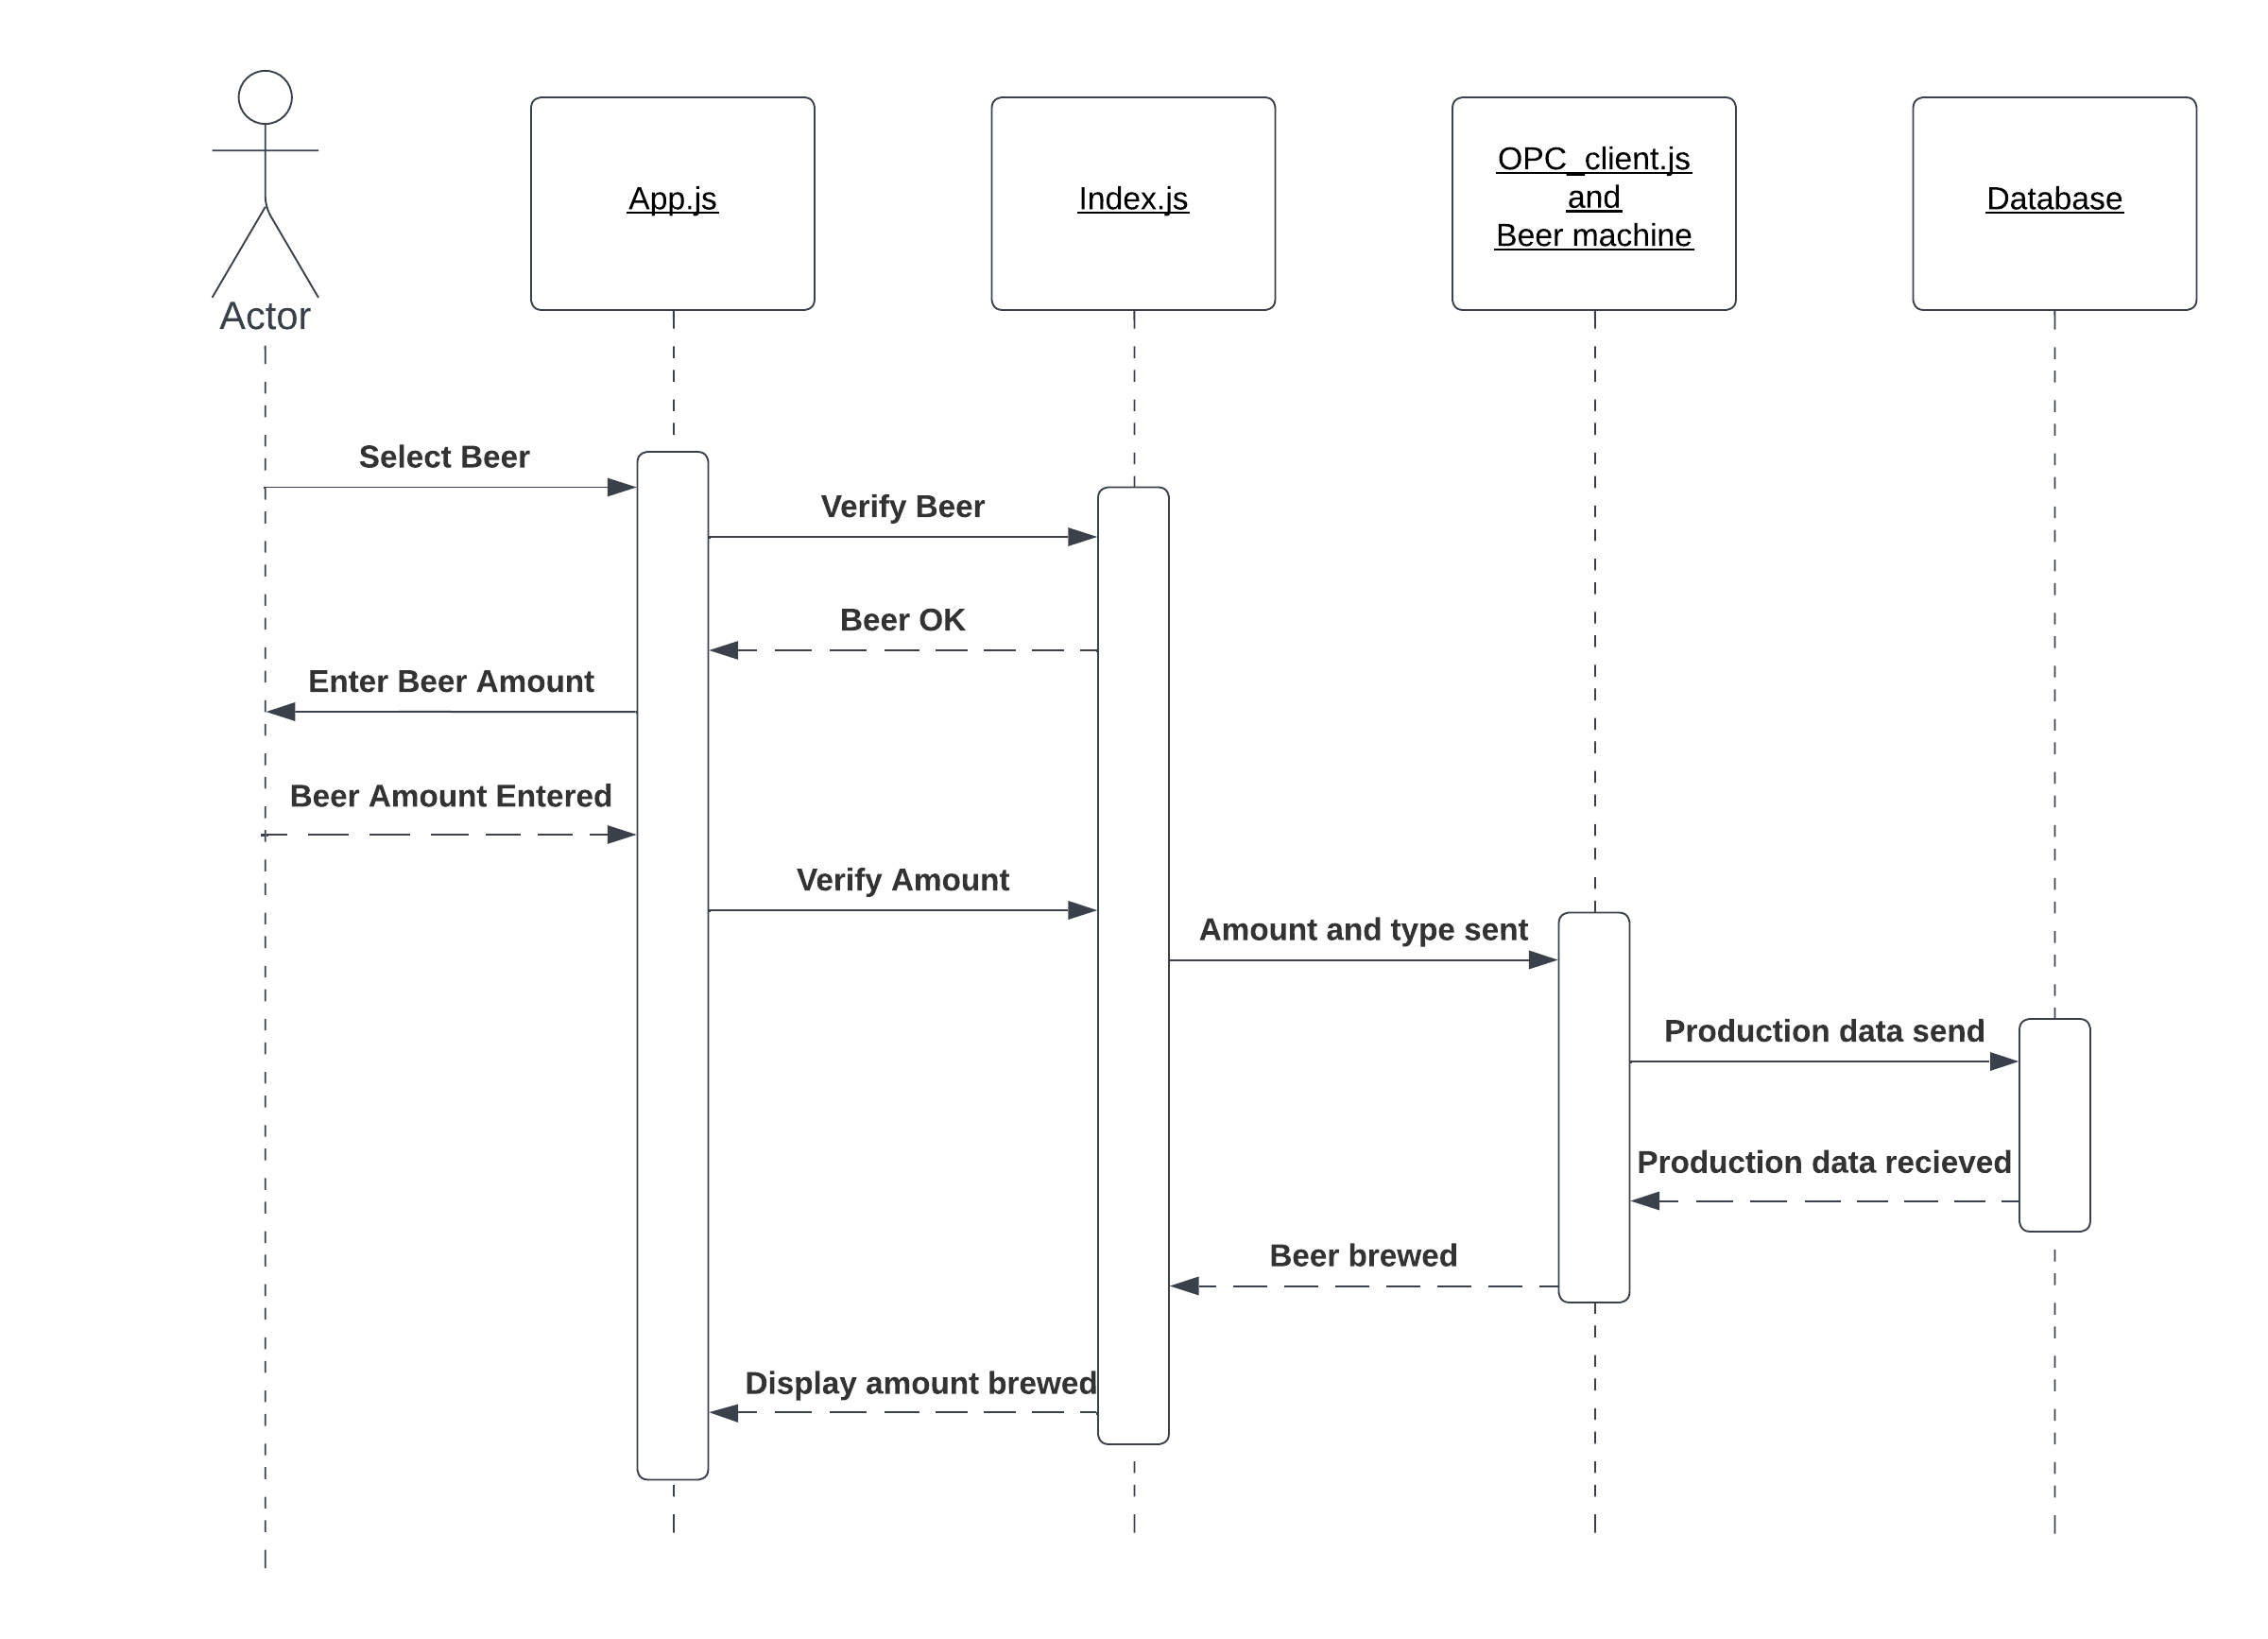
\includegraphics[width=1\textwidth]{img/SQdiagram_implementation.png}
        \caption{Sequence diagram of the system}
        \label{fig:SQdiagram_implementation}
    \end{figure}
\end{center}

Figure \ref{fig:SQdiagram_implementation} shows the sequence diagram of the system. The diagram shows the behaviour and workflow between the different components and how they react to input. When a user selects a beer from the user-friendly interface the frontend(App.jsx) it will send a request to the backend, where the backend will verify the selected beer, then the request is sent back to the frontend where the user can input the amount of beer he wants breewed. When the amount and type is selected, the brewing request is sent to the OPC or beer machine.
When the brewing is done, the data for the given batch production will be sent to the database, with data about the succes of the brewing, failures and etc. This data can be handled if needed to help optimize the brewing process. The client does not get this message it work internally in our automated system. The service will sent a message to the backend saying the beer is done, here the backend sent a request to the frontend where it user get displayed the beer type and amount brewed is a success.
Overall this is a simple representation of the sytems workflow, but it helps indicate the progress from selecting a beer to actually getting the product.

\subsubsubsection{Class diagram}

\begin{center}
    \centering
    \begin{figure}[H]
        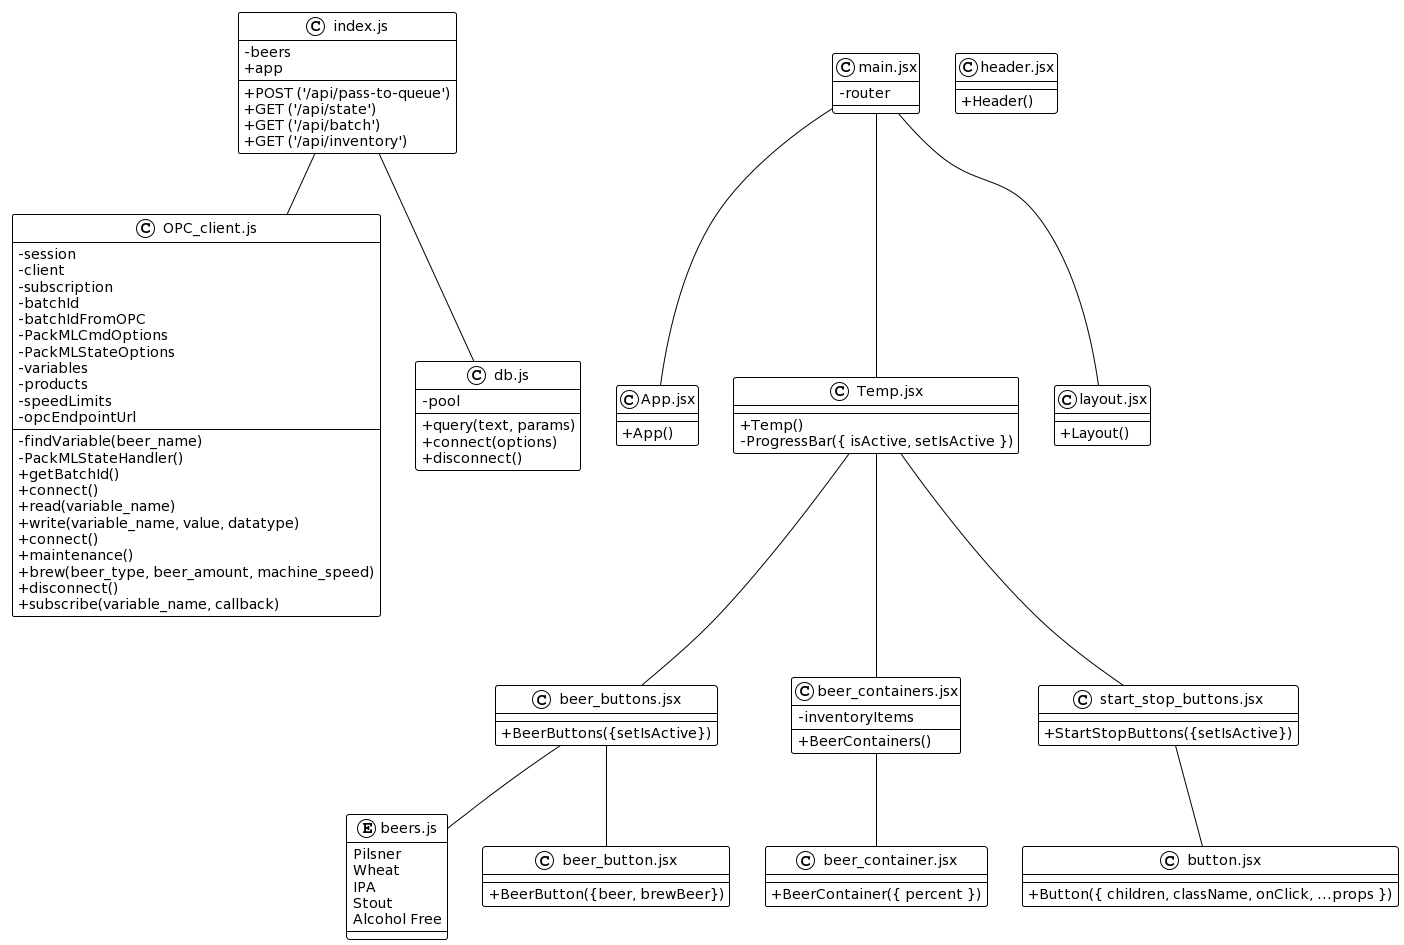
\includegraphics[width=1\textwidth]{img/class_diagram.png}
        \caption{Class diagram of the system}
        \label{fig:class_diagram}
    \end{figure}
\end{center}
Figure \ref{fig:class_diagram} shows the class diagram of the system. The diagram shows the different classes and how they are connected. The system is divided into three components, a dockerfile that boots up the backend, frontend and OPCUA-Client, we have the beer machine itself, and lastly the database which enables us to save data that is generated during the brewing process. This data collected can be accesed and help us understand and give improvements to the system.

\subsubsubsection{index.js}

The index.js file is responsible for our backend, which handles routing and requests. Currently we have the following endpoints
\begin{enumerate}
    \item {POST ('/api/pass-to-queue')}
    \item {GET ('/api/state')}
    \item {GET ('/api/batch')}
    \item {GET ('/api/inventory')}
\end{enumerate}

Our only \textit{POST} endpoint, which is the first in the list, is responsible for creating a brewing order. It recevies a body of type JSON with the keys \textit{'speed'},\textit{'amount'} and \textit{'type'}, which is the beer type. However the speed is not required. If there isn't any value entered, it will have a fallback of 10.
While running the brewing method, it will continously update the state, as we have subscribed to the node, that holds the stateCurrent value. If it isn't in \textit{execute}, which is the state that it is in, when it is brewing, it will brew. Otherwise if it is brewing (in execute state or 6 of value), then it will send an error to the user and not run that brewing order.
This way it can never brew if it is already brewing. \newline

Our 3 \textit{GET} endpoints is just for the client to receive data. Which is the state, batchId and inventory, respectively.
And all of these \textit{GET} endpoints are server-sent events (SSE). This means that the user will get the information streamed down continously. \newline

Our most essential API endpoint is our POST request, as it is the one to make a brewing order. Here is some of our code so show what is happening, when a user makes an order

\begin{center}
    \centering
    \begin{figure}[H]
        \begin{minted}[tabsize=2,breaklines]{javascript}
            app.post('/api/pass-to-queue', async (req, res) => {
                try {
                    // input validation code...
                    await opcuaClient.connect()
        
                    const state = opcuaClient.getStateCurrent()
                    if (state == opcuaClient.PackMLStateOptions.Execute) throw new Error('Brewing is not possible at the moment')
        
                    if (await opcuaClient.brew(beer_type, beer_amount, speed ?? 10)) {
                        // send beer type request to queue
                        res.status(200) // if ok, return status code OK
                        res.send({ status: 'ok' })
                    } else {
                        res.status(418) // refuse to brew
                        res.send({ status: 'error', error: 'Brewing failed' })
                    }
                } catch (error) {
                    console.error(error)
                    res.status(500).send({ error: error.message, status: 'error' })
                }
            })
        \end{minted}
        \caption{Code for our \textit{POST} endpoint}
        \label{fig:pass_to_queue_api}
    \end{figure}
\end{center}
Figure \ref{fig:pass_to_queue_api} shows the code for our \textit{POST} endpoint. It is responsible for making a brewing order. It first checks if the state is in \textit{execute}, which is the state it is in, when it is brewing. If it is, then it will throw an error, as it is not possible to brew, when it is already brewing. Otherwise it will brew the beer, and if it is successful, it will send a status code of 200, which means OK. Otherwise it will send a status code of 418, which means I'm a teapot. This is just a joke. But it is a valid status code, so we decided to use it.

\subsubsubsection{OPC\_client.js}


\begin{center}
    \centering
    \begin{figure}[H]
        \begin{minted}[tabsize=2,breaklines,breakanywhere,samepage]{javascript}
            brew: async (beer_type, beer_amount, machine_speed) => {
                try {
                    if (beer_type === undefined || !beer_amount || !machine_speed) return false                    

                    if (Object.values(products).indexOf(beer_type) === -1) return false

                    const maxMachineSpeedForBeerType = speedLimits[beer_type]

                    if (machine_speed < 0 || machine_speed > maxMachineSpeedForBeerType) return false

                    ... 

                    let state = await module.exports.read('StateCurrent')
                    if (state !== PackMLStateOptions.Execute) await PackMLStateHandler()

                    const currentStopReason = await module.exports.read('StopReason')
                    const needsMaintenance = currentStopReason === 10 || currentStopReason === 11

                    if (needsMaintenance) await module.exports.maintenence()

                    for (let node of nodesToWrite) {
                        const StopReason = await module.exports.read('StopReason')
                        if (StopReason === 10 || StopReason === 11) await module.exports.maintenence()
                        await module.exports.write(node.variable, node.value, node.dataType)
                    }

                    batchId++
                    await module.exports.write('SetBatchId', batchId, DataType.Float)

                    state = await module.exports.read('StateCurrent')
                    if (state !== PackMLStateOptions.Execute) await PackMLStateHandler()
                    return true
                } catch (err) {
                    console.error('An error occurred while brewing:', err)
                    return false
                }
            },
        \end{minted}
        \caption{Code for our brew method}
        \label{fig:opc_client_brew}
    \end{figure}
\end{center}
Figure \ref{fig:opc_client_brew} shows the code for our beer brewing method. Initially, it validates essential parameters—beer type, amount, and machine speed—returning false if any are undefined or set to zero. Furthermore, it confirms the beer type's existence in the products object and checks if the machine speed falls within the acceptable range for that type. \newline

After these checks, it ensures the system is in the 'execute' state for brewing. If not, it triggers the PackMLStateHandler method. It also handles maintenance if the stop reason is 10 or 11, iterating through nodesToWrite to update data and managing the batch ID.\newline

Upon successful execution, it returns true. Any encountered errors prompt a false return.\newline
\section{Tests}

In our project we have developed tests.
This means that we started coding, making the features that we agreed on
and seeing if it works after they were developed.
In order to be certain that the quality is the same as before
and to ensure that we do not accidentally break something which would not be on purpose.
If it works, then we would make tests to ensure stability and robustness.
This is not the best way to do it, but it was the way we did it.
This also means that going forward and if it was a bigger project
we would ideally have to make tests before we started coding.
We have used the JavaScript test framework \textit{Mocha} for our tests.

\subsection{Unit Tests}

Unit tests are tests that are made to test the smallest parts of the code.
In practice this will lead to making tests of small isolated functions and methods.
This is done to ensure that the code is working as intended and that it is robust.
With the \textit{Mocha} test framework, we have made unit tests for the backend and the OPC-UA client.
However, we have not made unit tests for the frontend.
This is because it is a user interface and it is not as easy to test, and as the frontend is not the main focus of the project, we decided to not make unit tests for it.
It also means that the frontend is not as robust as the backend and OPC-UA client, and is more likely to break if something is changed.
The unit tests for the backend are made to test the endpoints and the functions that are used in the endpoints.
The unit tests for the OPC-UA client are made to test the connection to the OPC-UA server and the functions that are used to both send and get data from the server. \newline

\subsection{Machine Tests}
With all the information we have gathered, we now need to find the optimal speed for each beer type. The speed we will find will be the optimal speed for brewing the beer, in your own home. In our case,
we would like the fail rate to be as low as posssbile, because our stakeholders are primarily hobbysit brewers, and would like the quality of the beer to be as good as possbile.
We have made a test for each beer type, where we have tested the speed of the machine, and the fail rate of the machine. The fail rate is the amount of times the machine fails to brew the beer.
Using the gathered, we have made a graph for each type to help us optimize the perfect speed for the machine. \newline
The way we gathered the data was using our own brew function, where we could select the beer type, beer amount as well as the speed of the machine. On each test, we have different amounts of beers brewed, this is because we only want the best fail rate possbile, and the amount of beers does not impact the fail rate only the machine speed does.
We made a graph of all the data gathered from the test, on the X-axis we have the speed of the machine, and on the Y-axis we have the fail rate. \newline

\subsubsection{Machine speed calculation}
From the data we have gathered from the tests, we made calculations for each individual beer type, and the graph made from the data, as well as a fail rate of 0.99, 
which leaves us with a 1\% fail rate. Now that we have all the numbers, we need to calculate the optimal machine speeds for the brewing of each beer type. \newline
From the tendency line of the graph, we got an equation that we can use to calculate the optimal speed for each beer type. The eqauations differentiates from each other. The eqaution used is based on the line that is closets to the data points. which is where R2 is the closests to 1, which can be seen in each graph. \newline
From the given equation, and the fail rate of 0.99, we can calcualte the optimal speed by setting 0.99 as the fail rate, and then solve for the speed. This is done by putting the fail rate into the equation, and solve each equation for the speed which is the x value in each equation. \newline
This is done on each graph, and the results can be seen below in the following chapters of each beer type. \newline



\subsubsection{Pilsner}
For the Pilsner test, we have tested the machine with different speeds: 600, 500, 400, 300, 200. The amount of beers brewed for each test was 1000.

\begin{center}
    \centering
    \begin{figure}[H]
        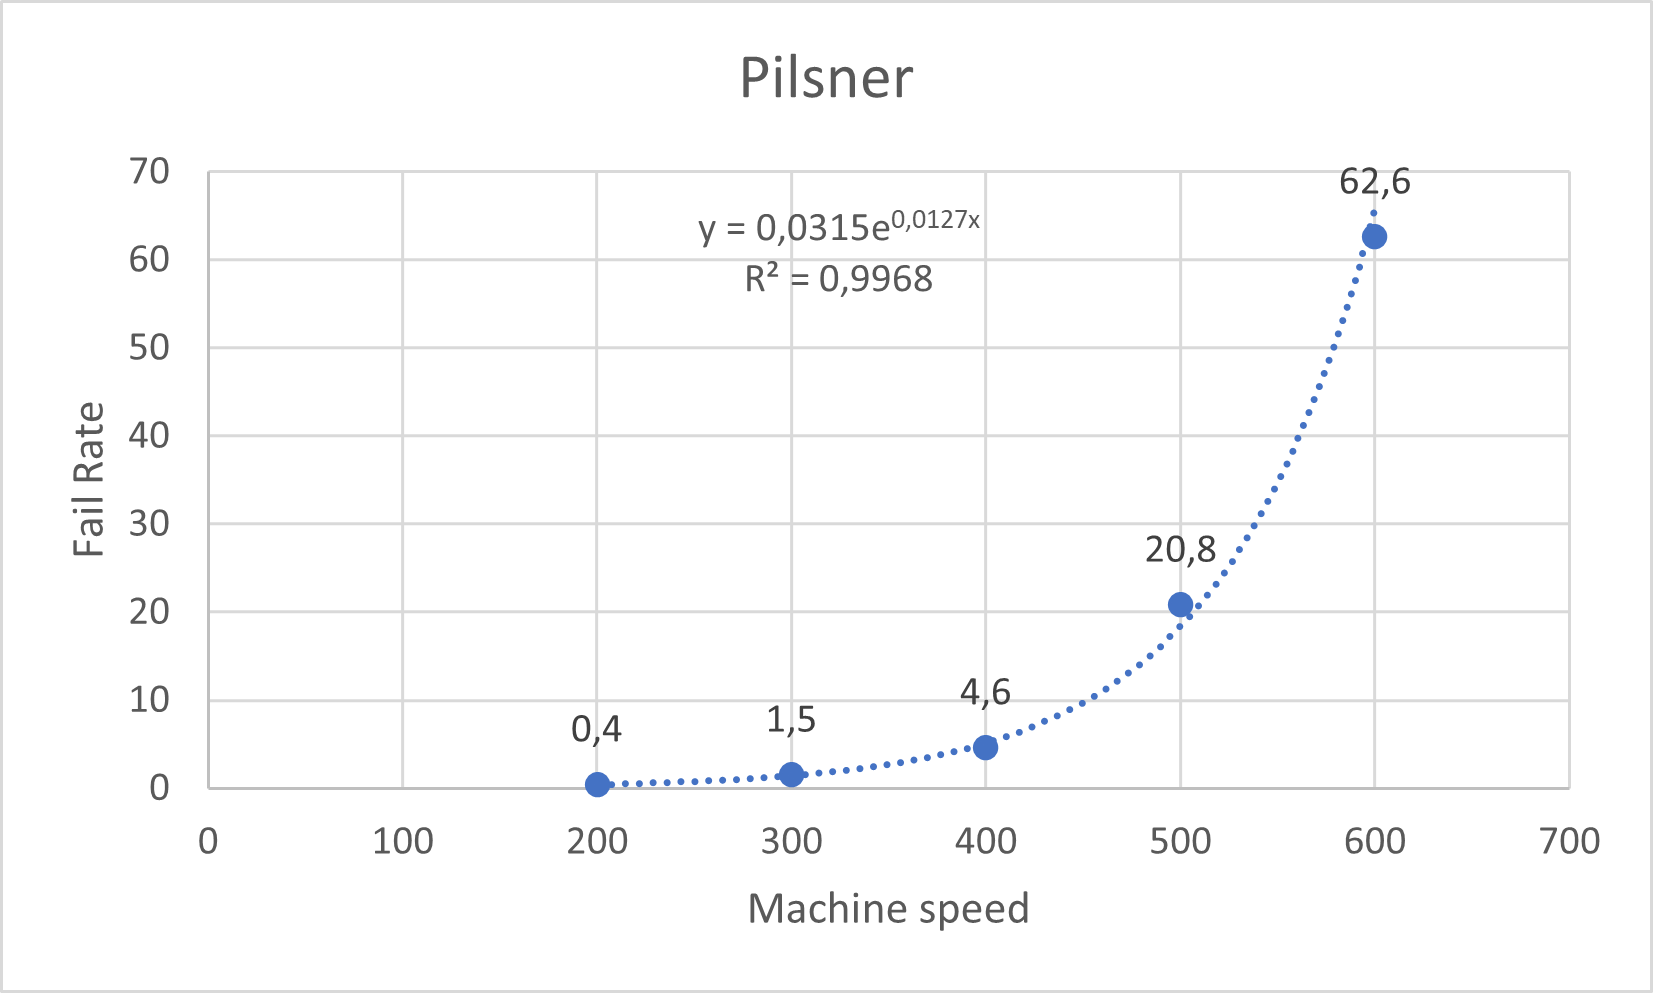
\includegraphics[width=1\textwidth]{img/Pilsner_graph.png}
        \caption{Graph over data from Pilsner tests}
        \label{fig:Pilsner_graph}
    \end{figure}
\end{center}

Figure \ref{fig:Pilsner_graph} shows the graph over the data from the Pilsner tests, with the R2 value and the equation for the line to find the optimal speed for the machine. \newline
From the calutaion made for Pilsner, we got the following machine speed after solving the equations which was 263. This is the optimal speed for brewing Pilsner for our hobbyists. \newline

\subsubsection{Wheat}
For the Wheat test, we used the following speeds: 300, 250, 200, 150, 100. The amount of beers brewed for each test was 500.

\begin{center}
    \centering
    \begin{figure}[H]
        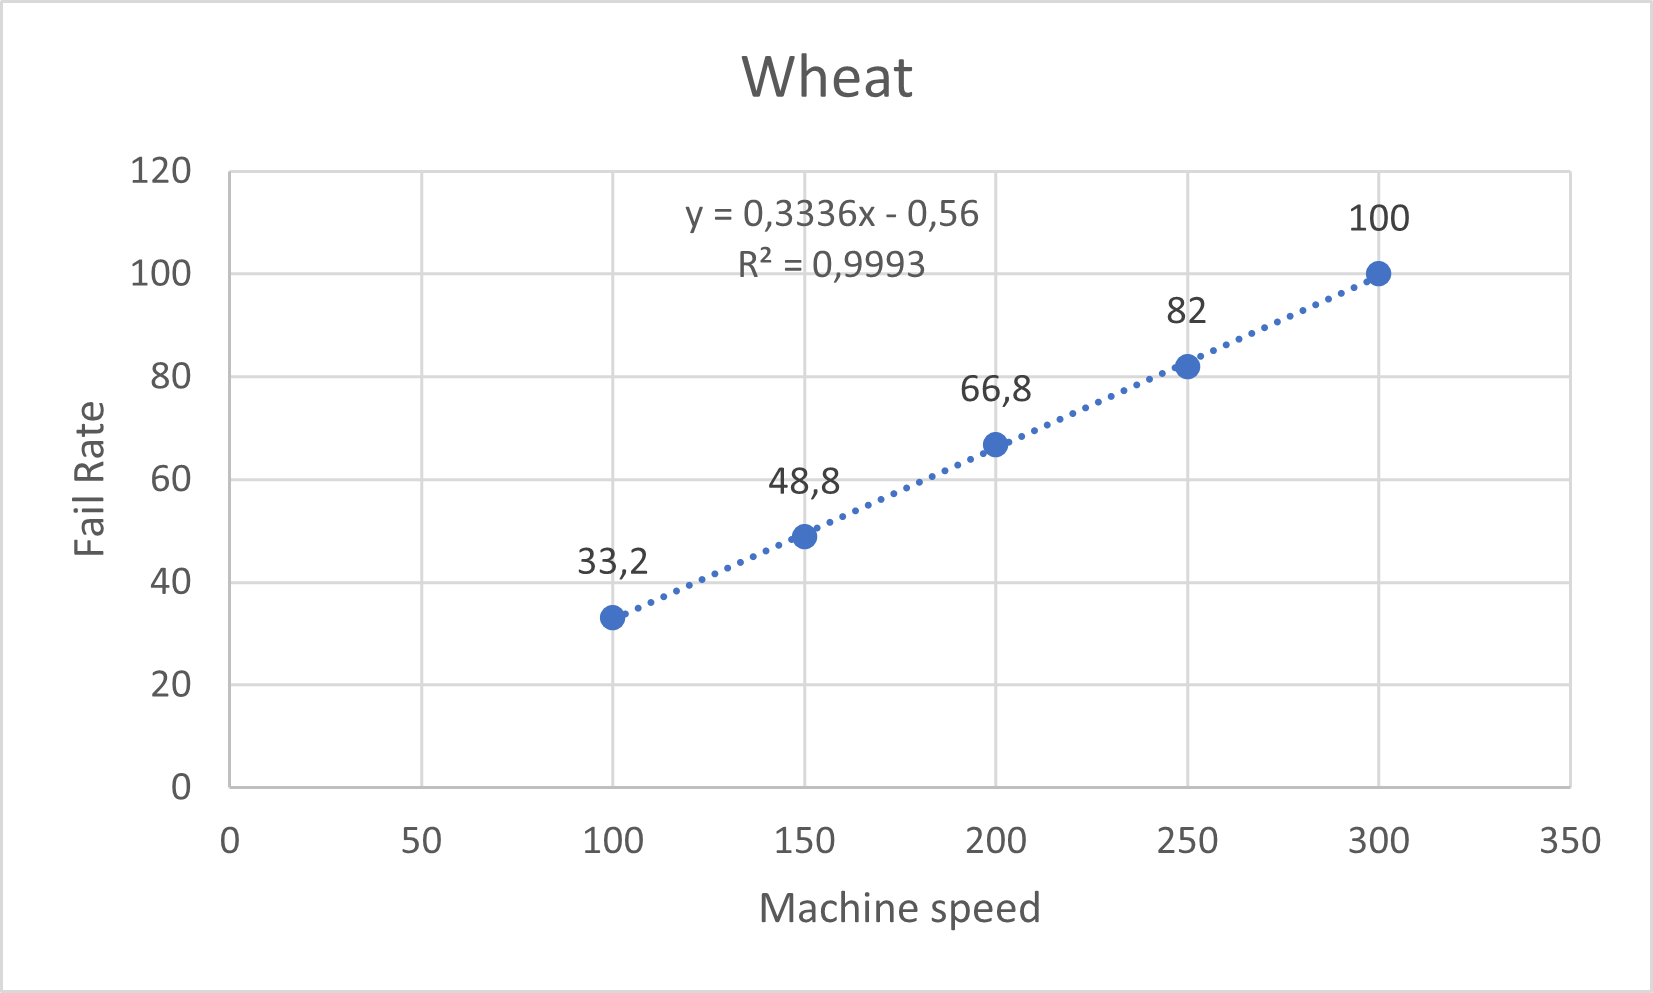
\includegraphics[width=1\textwidth]{img/Wheat_graph.png}
        \caption{Graph over data from Wheat tests}
        \label{fig:Wheat_graph}
    \end{figure}
\end{center}

Figure \ref{fig:Wheat_graph} shows the graph over the data from the Wheat tests, with the R2 value and the equation for the line to find the optimal speed for the machine. \newline
From the calutaion made for Wheat, we got the following machine speed after solving the equations which was 5. This is the optimal speed for brewing Wheat for our hobbyists. \newline

\subsubsection{IPA}
For the IPA test, we used the following speeds: 150, 125, 100, 75, 50. The amount of beers brewed for each test was 250.

\begin{center}
    \centering
    \begin{figure}[H]
        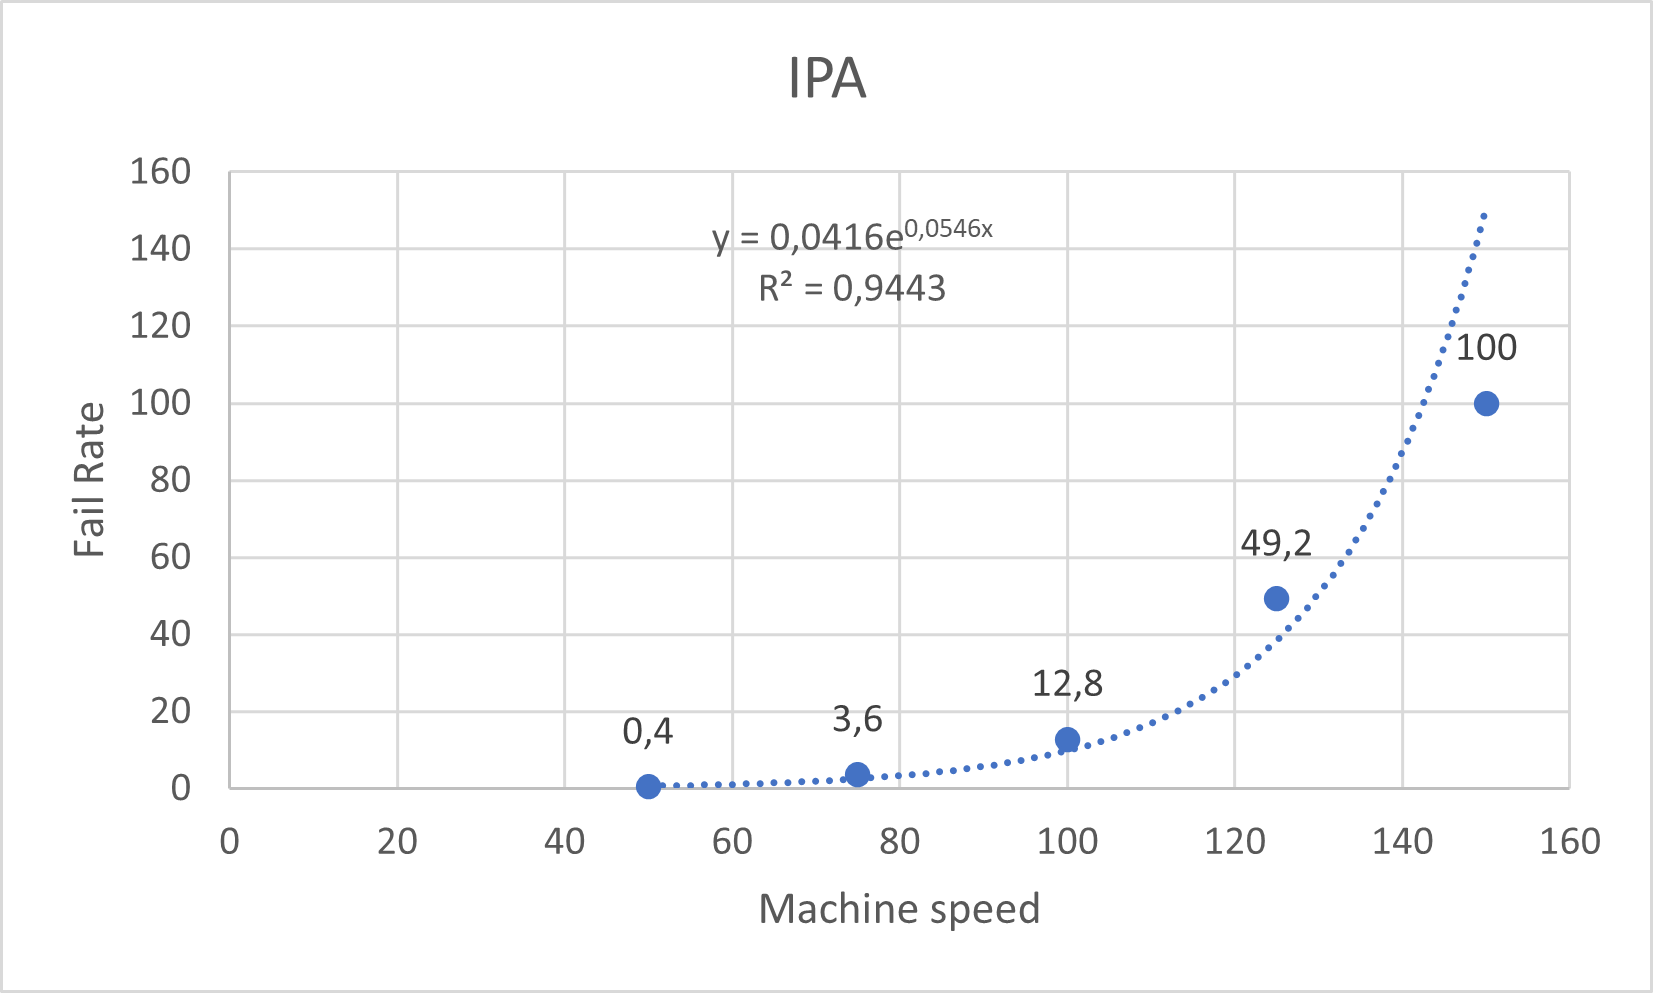
\includegraphics[width=1\textwidth]{img/IPA_graph.png}
        \caption{Graph over data from IPA tests}
        \label{fig:IPA_graph}
    \end{figure}
\end{center}

Figure \ref{fig:IPA_graph} shows the graph over the data from the IPA tests, with the R2 value and the equation for the line to find the optimal speed for the machine. \newline
From the calutaion made for IPA, we got the following machine speed after solving the equations which was 58. This is the optimal speed for brewing IPA for our hobbyists. \newline

\subsubsection{Stout}
For the Stout test, we used the following speeds: 200, 175, 150, 125, 100. The amount of beers brewed for each test was 300.

\begin{center}
    \centering
    \begin{figure}[H]
        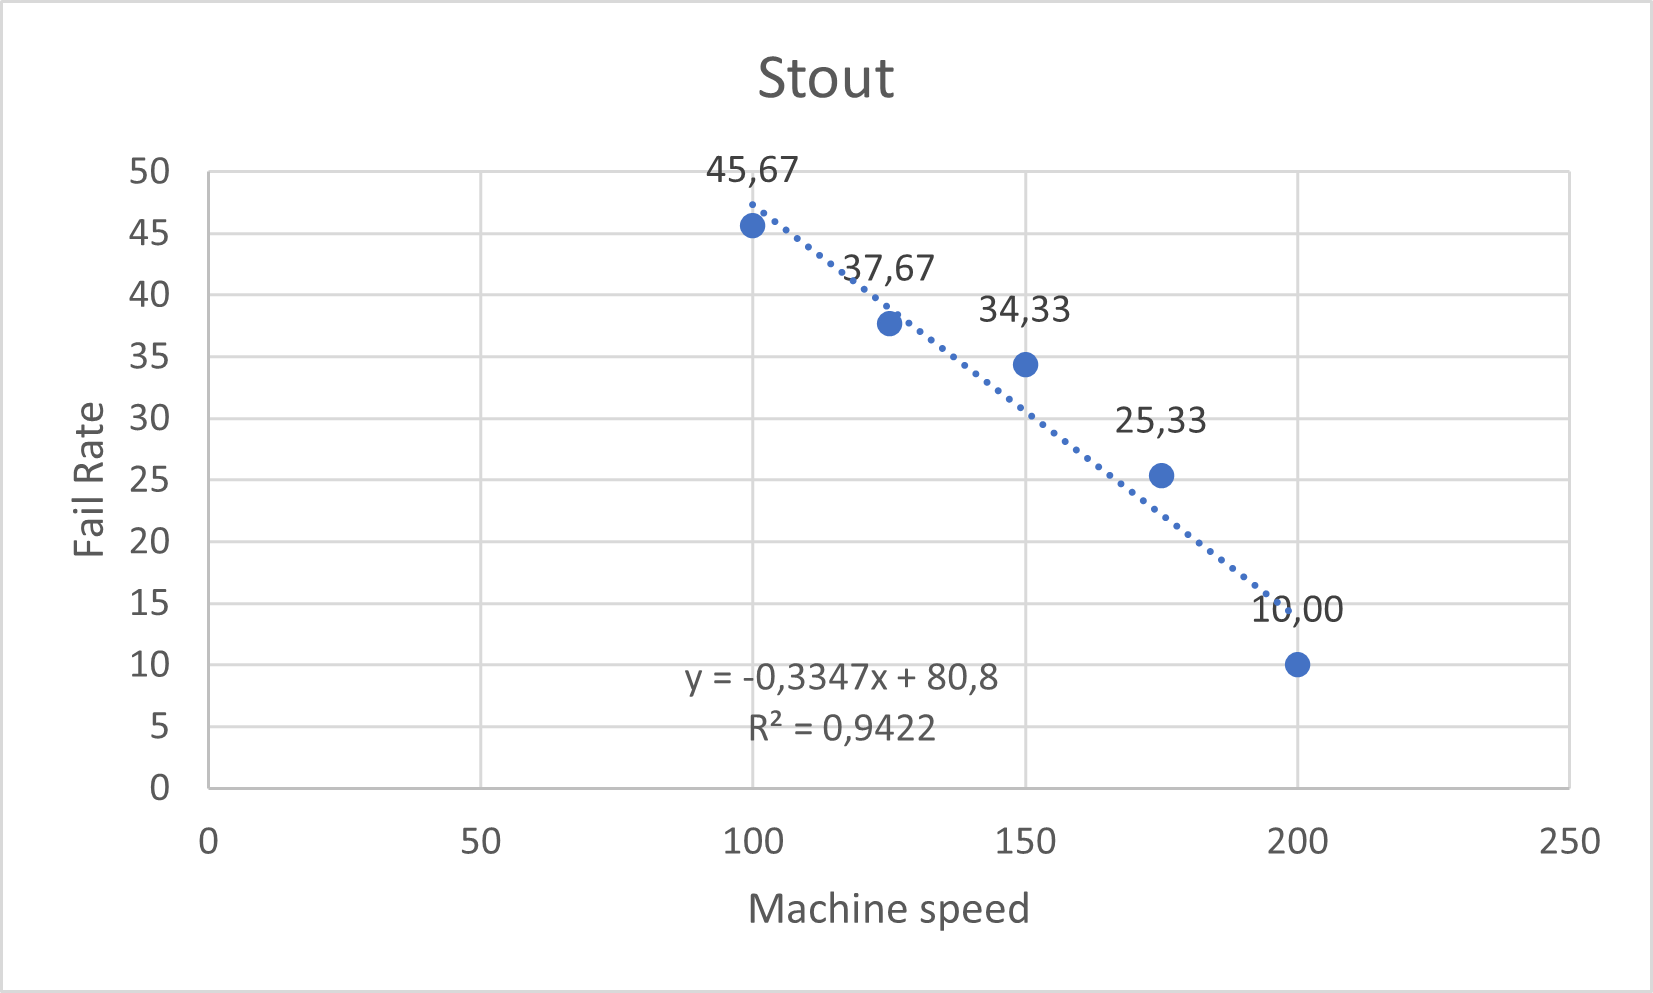
\includegraphics[width=1\textwidth]{img/Stout_graph.png}
        \caption{Graph over data from Stout tests}
        \label{fig:Stout_graph}
    \end{figure}
\end{center}

Figure \ref{fig:Stout_graph} shows the graph over the data from the Stout tests, with the R2 value and the equation for the line to find the optimal speed for the machine. \newline
From the calutaion made for Stout, we got the following machine speed after solving the equations which was 238. This is theoretically, the best machine speed for brewing Stout, but the problem is that the machine only allows the machine speed for Stout to be 200.
In our case the calculated machine speed is over the limit of the machine. This cannot be done, because the machine will give us a failure, so if we want the hobbyists to have the lowest fail rate possbile, they need to brew Stout with a machine speed of 200, which is the maximum. \newline

\subsubsection{Ale}
For the Ale test, we used the following speeds: 100, 80, 60, 40, 20. The amount of beers brewed for each test was 200.

\begin{center}
    \centering
    \begin{figure}[H]
        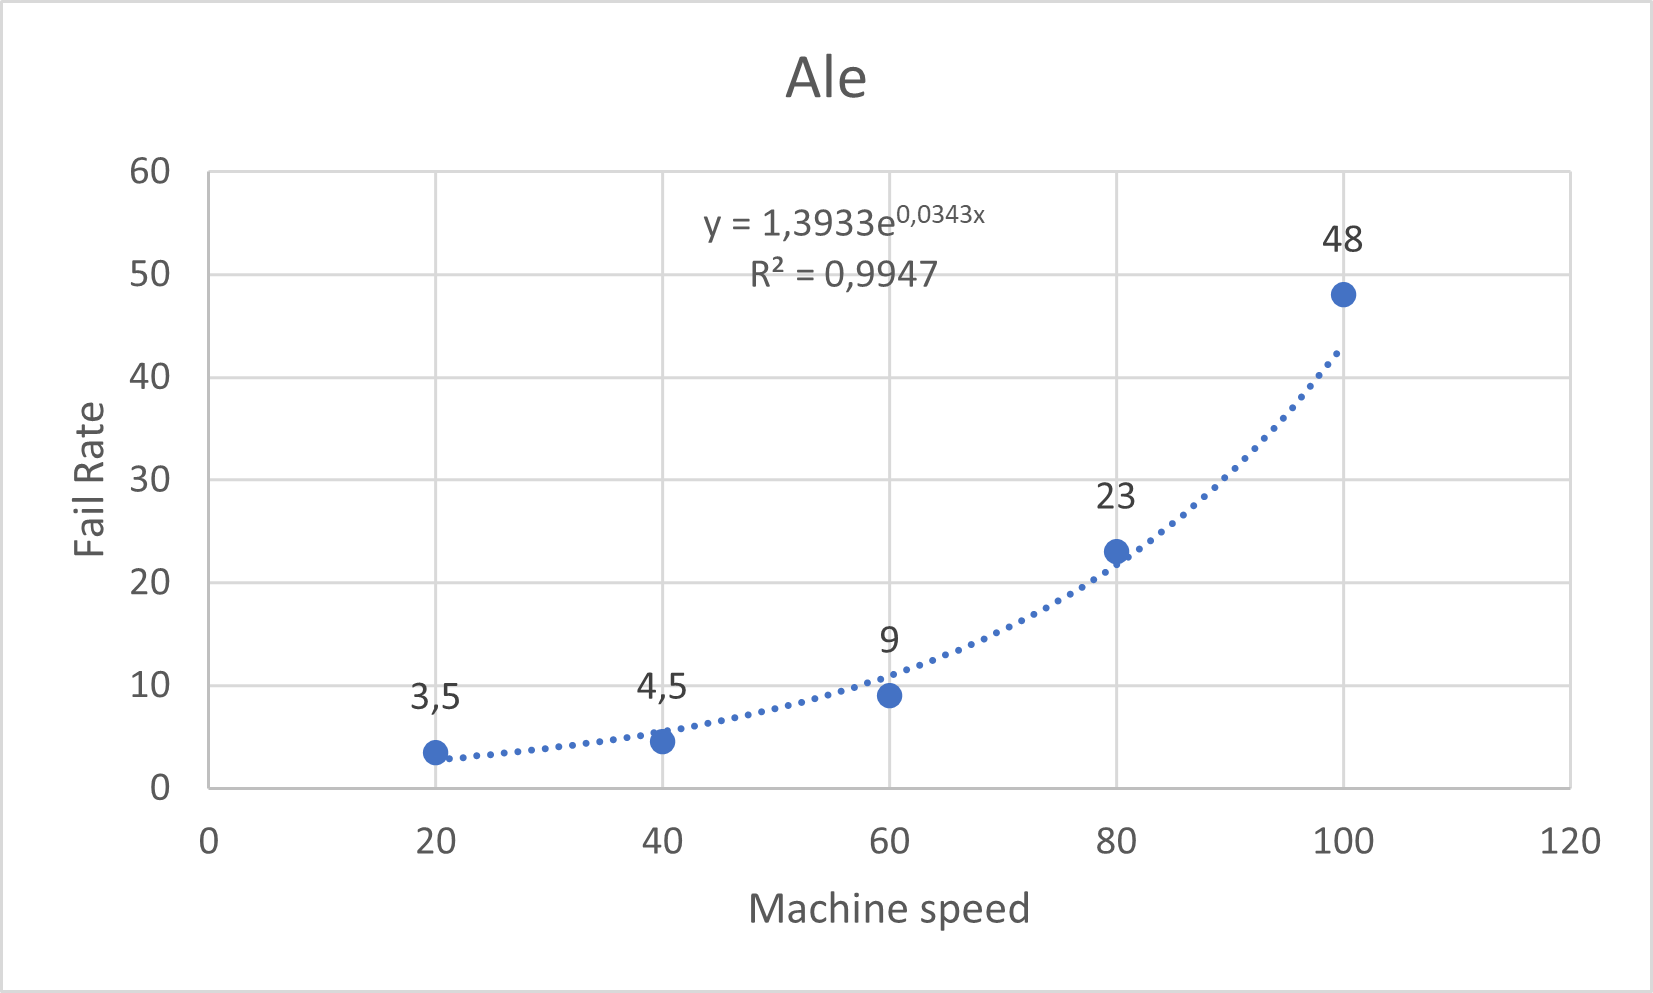
\includegraphics[width=1\textwidth]{img/Ale_graph.png}
        \caption{Graph over data from Ale tests}
        \label{fig:Ale_graph}
    \end{figure}
\end{center}

Figure \ref{fig:Ale_graph} shows the graph over the data from the Ale tests, with the R2 value and the equation for the line to find the optimal speed for the machine. \newline
From the calutaion made for Ale, we got the following machine speed after solving the equations which was -10. This indicates the best speed for brewing Ale, but it is not possibly to select this speed because it a negative value and the machine only allows for postive ones. 
So for our hobbysits to have the lowest fail rate as possbile, they would need to brew the Ale with a machine speed of 1, which is the slowest machine speed possbile, but would give the lowest fail rate. \newline


\subsubsection{Alcohol Free}
For the Alcohol Free test, we used the following speeds: 125, 100, 75, 50, 25. The amount of beers brewed for each test was 225.

\begin{center}
    \centering
    \begin{figure}[H]
        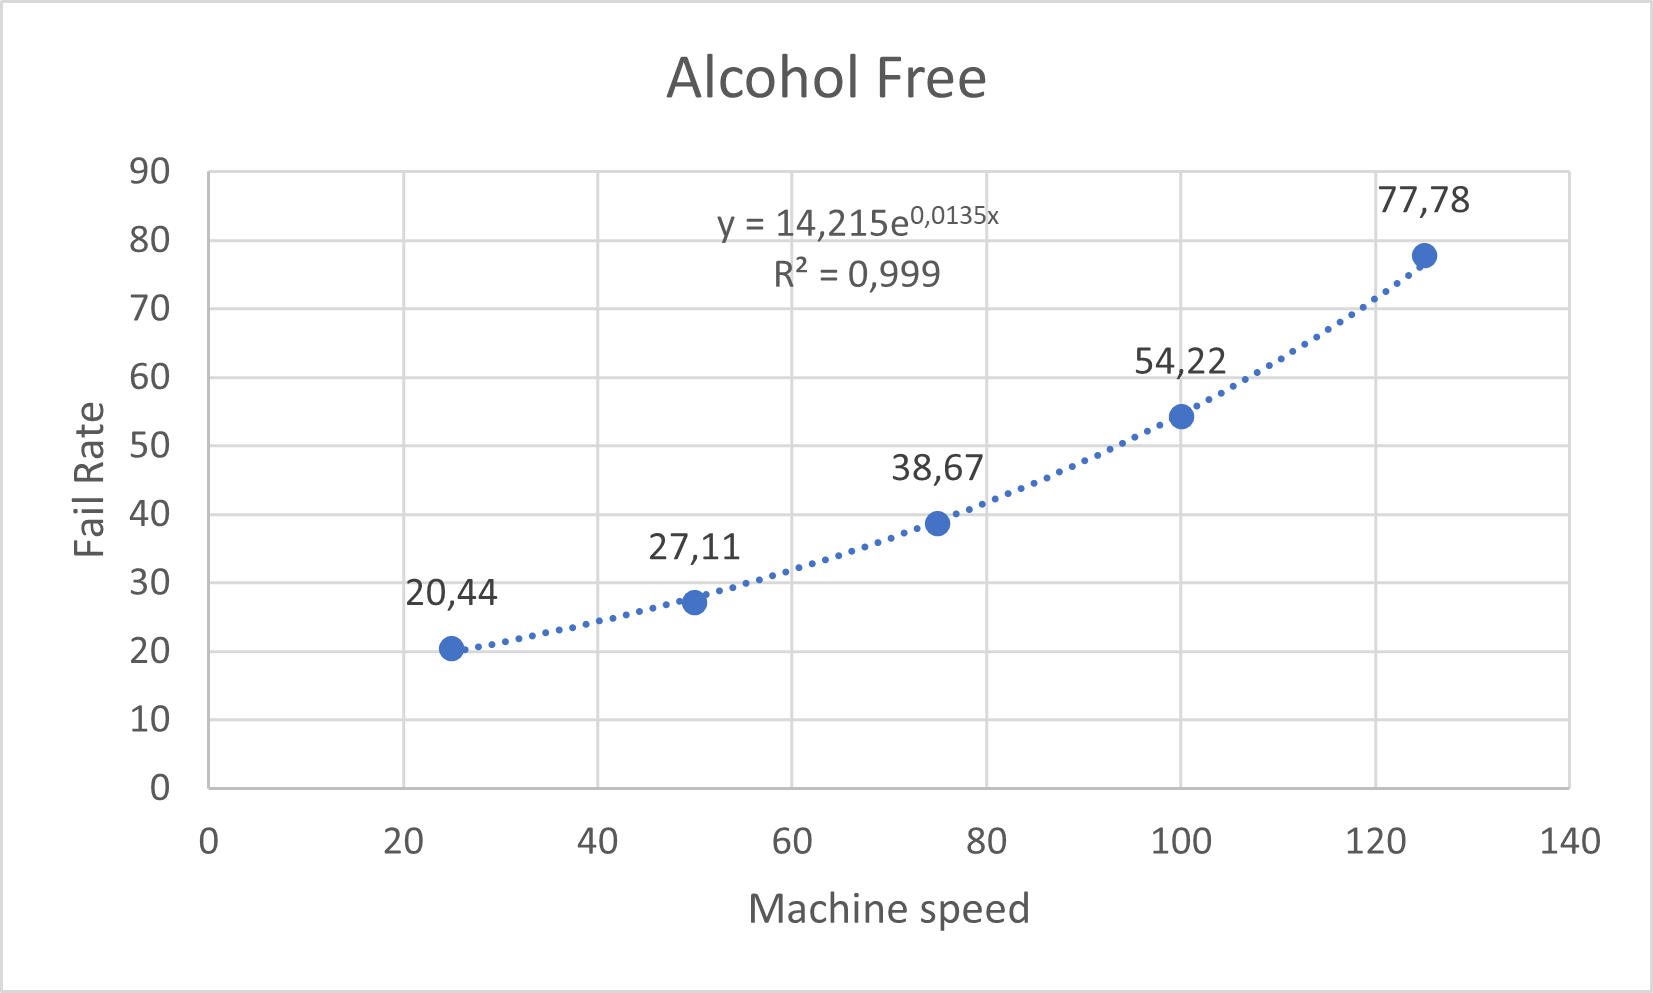
\includegraphics[width=1\textwidth]{img/AlcoholFree_graph.png}
        \caption{Graph over data from Alcohol Free tests}
        \label{fig:AlcoholFree_graph}
    \end{figure}
\end{center}

Figure \ref{fig:AlcoholFree_graph} shows the graph over the data from the Alcohol Free tests, with the R2 value and the equation for the line to find the optimal speed for the machine. \newline
From the calculation made for Alcohol Free, we got the following machine speed after solving the equations which was -198. Again we have a negative value, so the best speed for brewing the Alcohol Free beer is 1. \newline
\section{Discussion}

\subsection{Results}
\subsubsection{Achievements}
We managed to create a very thorough backend part for our application,
with all the functionality for automating the beer brewing process.
The frontend we've created is simple, but is able to communicate with the backend,
and allows the user to start the brewing process, and monitor the current inventory.

\subsubsection{Limitations}
\subsubsubsection{Machine Speed Limitations}
The requirements we set for the failure rate,
is not possible to achieve on all the beer types,
as some require speeds outside the limitations set by the machine.

\subsubsection{Collaboration and Communication}
\subsubsubsection{Meetings}
Each thursday we scheduled a meeting on campus between 10:00 and 14:00,
to explain any doubts about code, or questions about writing the report.
This was done so everyone had some understanding of all the aspects 
of the codebase, and the report.


\subsubsubsection{Communication}
We had a group chat on messenger, where we would write in case we were late,
or sick.
Besides that we had a discord for sharing code, doing voice calls in case 
we didn't show up at the meeting, or had questions about the code 
outside of the scheduled meeting times.

\subsubsection{Workflow}
For our workflow we used some aspects of the scrum methodology, such as splitting the work into different sprints, and having a product backlog.
This helped splitting the tasks into manageable chunks, which could be completed in a single sprint.
Whenever a task in the sprint was completed, the code would be pushed to our git repository,
to make sure we all had a log of what was done, and had access to the code.

\subsection{Future Improvements}
\subsubsection{Frontend}
The frontend is not fully functional, as the only two features currently implemted, are the brewing process, and the inventory.
We could still have the stop/start buttons implemented, and the ability to brew more than a single beer at a time.

\section{Conclusion}
Based on the analysis we came to the conclusion that our target group is hobbyists or home brewers.
We have also concluded that the most important features for our target group is the ability to simplify the brewing process and
make it easier and less time consuming, this is necessary since brewing process is very complex and time consuming
as we do not expect our users to have any prior experience or expertise in brewing.\newline

With the help of the analysis, requirements for the project was made.
Based on these requirements we made a design for the system.
In the design we decided to use a client-server architecture, where the client is a web application and the server is a REST API.
The REST API is used to communicate with the database and the OPC-UA client.
The OPC-UA client is used to communicate with the machine, where the brewing process takes place.
We also made a database for storing the order with the beer type, the amount of beers and the timestamp.\newline

The implementation of the system was made with the design in mind.
In the web application we decided to use a single page application (SPA) with the UI library React,
since it makes it easier to update the UI without having to reload the page.
We decided to go for a backend with Node.js instead of Java, because it is easier to use and faster to develop with than Java.
The Milo OPC-UA library in Java is running on Java 8, which is a very old version.
The REST API was made with the framework Express and the OPC-UA client was made with the library node-opcua.
The database was made with the database management system (DBMS) PostgreSQL, using the pg library.\newline

To make sure our system worked as we intended, we tested the system.
We made unit tests for the Express REST API backend and for the OPC-UA client.
We also tested each of the beer types with different speeds and observed the fail rate,
as one of our requirements was to aim for optimal speed for each beer type.
From the data gathered, graphs were made for each beer type together with a regression line.
Based on that regression line we solved for having a failrate of 1\%.
As negative speeds are not possible we decided to use 1 as the speed for Ale and Alcohol Free.\newline

Overall, we have made a simplified and automated system for hobbyists and home brewers,
that has been tested and optimized. The system uses the client-server architecture with a Node.js REST API backend,
using an OPC-UA client, which is connected to the OPC-UA server, and React frontend together with storing the orders in a PostgreSQL database.

\newpage

\printbibliography

\end{document}
